\section{Виртуализация}
\subsection{Введение}
У пользователей Linux и Mac иногда возникает проблема с запуском программ под Windows.
Или часто разработчики хотят протестировать или запустить программу написанную для какого-то другого девайса на своем компьютере.
Для решения этой проблемы придумали виртуализацию.

Виртуализация — предоставление набора вычислительных ресурсов или их логического объединения, абстрагированное от аппаратной реализации, и обеспечивающее при этом логическую изоляцию друг от друга вычислительных процессов, выполняемых на одном физическом ресурсе.

Машина, на которой запускается весь процесс называют host системой, а которая работает в виртуальном окружении guest системой.
Например, если запустить винду на машине с линуксом, то хост -- линукс, а гость -- винда.
Гипервизор занимается созданием виртуальных машин и их управлением.
Он обеспечивает изоляцию систем друг от друга, защиту и безопасность, разделение ресурсов.
Более просто это маленькая операционная система, которая может управлять памятью, сетью и остальным.

Для виртуализации применяются разные подходы и в основных вида --- аппаратная и программная.

\subsection{Кольца защиты}
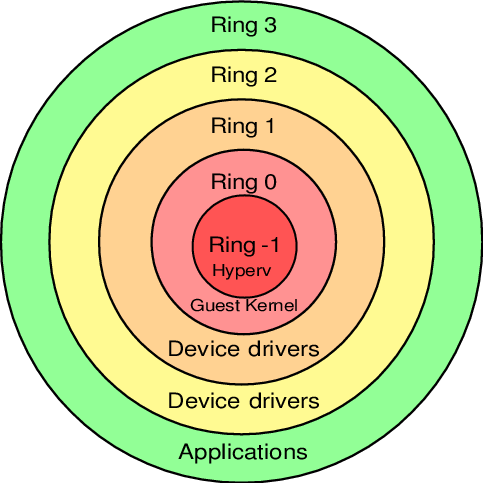
\includegraphics[scale=0.5]{protection-rings}

Бинарный программный код на процессорах работает не просто так, а располагается на разных уровнях (кольцах / Protection rings) с разными уровнями доступа к данным, от самого привилегированного (Ring 0), до самого ограниченного, зарегулированного (Ring 3).

Операционная система (ядро ОС) работает на Ring 0 (kernel mode) и может делать с любыми данными и устройствами все, что угодно.
Пользовательские приложения работают на уровне Ring 3 (user mode) и не в праве делать все, что захотят, а вместо этого каждый раз должны запрашивать доступ на проведение той или иной операции (таким образом, пользовательские приложения имеют доступ только к собственным данным и не могут «влезть» в «чужую песочницу»).

С появлением Intel VT-x / AMD SVM, был создан специальный новый уровень Ring -1. И теперь на нем работает гипервизор, а гости работают на Ring 0 и получают привилегированный доступ к CPU.

\subsection{Аппаратная виртуализация}
Аппаратная виртуализация(hardware virtualization) --- виртуализация с поддержкой специальной процессорной архитектуры.

В этом случае гипервизор работает напрямую с железоом без хост системы.

В качестве примера можете посмотреть на Intel Virtualization Technology (Intel VT) и AMD virtualization (AMD-V).
%Кажется это динамическая программная виртуализация
%Например, Apple выпустила новые чипы M1 работающие на ARM-архитектуре.
%Чтобы запускать приложения, которые были скомпилированы под прошлые версии компьютеров запускается аппаратная виртуализация Rosetta 2.

\subsection{Программная виртуализация}
Программная виртуализация (software virtualization) --- это виртуализация, которая происходит на уровне ядра ОС.

В этом случае гипервизор работает через основную хост-систему.

Например, новые чипы стоят и на новых iPad/iPhone, и на новых Mac, поэтому есть возможность запускать приложения под мобильные девайсы на компютерах и менять управление на уровне ОС.

Программная виртуализация так же может быть разных тпиов:
\begin{itemize}
  \item Динамическая --- подмена инструкций "на ходу"
  \item Паравиртуализация --- ядро гостевой системы незначительно модифицируется и использует гипервизор через api
  \item Встроенная
\end{itemize}

\subsection{Виртуализация в Linux}
Kernel-based Virtual Machine (KVM) --- это решение для виртуализации, встроенное прямо в ядро Linux, не уступающее остальным решениям в функциональности и превосходящее их в удобстве использования.

Создатели KVM изначально сфокусировались на поддержке аппаратной виртуализации и не стали переизобретать многие вещи.
Гипервизором здесь выступает ядро Linux.
Каждая виртуальная машина KVM --- это всего лишь отдельный Linux процесс с некоторыми наворотами для безопасности.
Начиная с версии ядра 2.6.20 KVM является основной составляющей Linux.

Несмотря на то, что KVM использует аппаратную виртуализацию, для некоторых драйверов I/O устройств KVM может использовать паравиртуализацию, что обеспечивает прирост производительности для определённых сценариев использования.

\subsection{Qemu}
QEMU (Quick Emulator) – эмулятор различных устройств, который позволяет запускать операционные системы, предназначенные под одну архитектуру на другой.
Кроме процессора, QEMU эмулирует различные периферийные устройства: сетевые карты, HDD, видео карты, PCI, USB и пр.

Если коротко, то инструкции/бинарный код (например, ARM) конвертируются в промежуточный платформонезависимый код при помощи конвертера TCG (Tiny Code Generator) и затем этот платформонезависимый бинарный код конвертируется уже в целевые инструкции/код (например, x86).

По сути, вы можете запускать виртуальные машины на QEMU на любом хосте, даже со старыми моделями процессоров, не поддерживающими Intel VT/AMD.
Однако в таком случае, это будет работать весьма медленно, в связи с тем, что исполняемый бинарный код нужно перекомпилировать на лету два раза, при помощи TCG.

Т.е. сам по себе QEMU крутой, но работает очень медленно.

Пример компиляции и запуска простого кода с Qemu:
\begin{lstlisting}
# Compile with required architecture arguments
> /opt/arm-gcc/bin/arm-linux-gnueabi-gcc -marm -o program hello.c
# Execute via qemu
> qemu-arm -L /opt/arm-sysroot ./program
\end{lstlisting}

\subsection{Virtaulbox}
Virtualbox это еще одна утилита для виртуализации.
VirtualBox запускает гостя на 3 уровне доступа (как обычный пользователь) и чтобы ошибки не могли повлиять на хост все команды с уровнем 0 заменяются на 1.
В случаях, когда mapping VB не справляется запускается qemu, поэтому он может работать достаточно долго.

Основной use-case virtualbox это поставить другую ось на текущую.
С этим можно справиться через GUI.

Также отмечу, что есть удобные утилиты использующие virtualbox, например, vagrant.

